\subsubsection{30.11.14}

\begin{enumerate}
	\item Время начала и окончания собрания:
	14:00 - 20:00
	\item Цели собрания:
	\begin{enumerate}
		\item Создать новый механизм захвата мячей.
		
		\item Испытать новый захват в действии.
		
	\end{enumerate}
	\item Проделанная работа:
	\begin{enumerate}
		\item На ось захвата мячей были установлены новые лопатки из пластиковых бутылок взамен стяжек.
		
		\begin{figure}[H]
			\begin{minipage}[h]{0.2\linewidth}
				\center  
			\end{minipage}
			\begin{minipage}[h]{0.6\linewidth}
				\center{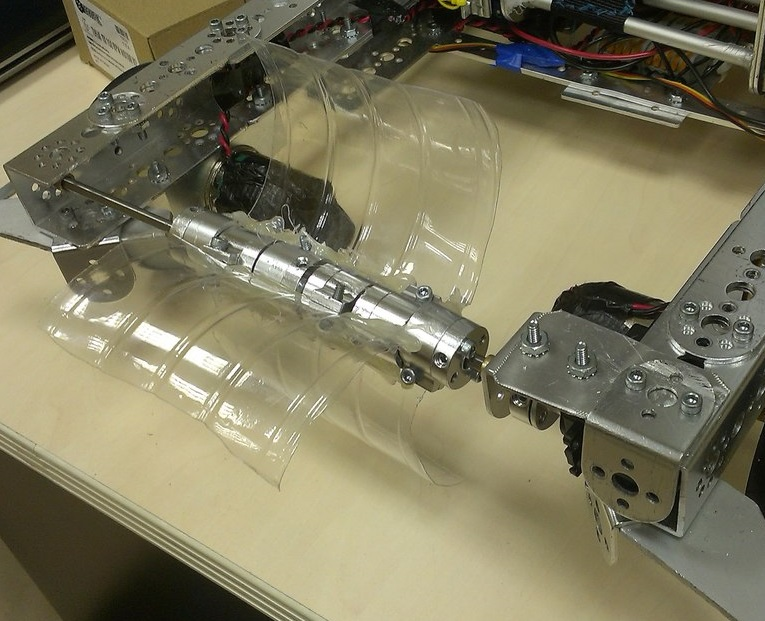
\includegraphics[scale=0.25]{days/30.11.14/images/01}}
				\caption{Захват мячей изменен}
			\end{minipage}
		\end{figure}
		
		\item Испытания.
		
		\item В связи с тем, что лопатки нового захвата более жесткие, поперечное ребро жесткости, установленное в передней части робота, которое ранее не мешало движению стяжек, сегодня было демонтировано. Вместо него было решено установить П-образное ребро жесткости, горизонтальная перекладина которого была бы расположена выше области действия захвата и не мешала бы его работе. Эта конструкция сегодня реализована. не была.
		
		\item Из-за того, что ось захвата мячей была расположена слишком низко, захвату требовалось много времени и усилий чтобы протолкнуть большой мяч. Чтобы улучшить работу захвата, было решено увеличить клиренс передней части робота (теперь клиренс всех колес робота был максимальным). После увеличения клиренса захват больше не испытывал проблем с большим мячом.
		
	%	\begin{figure}[H]
	%		\begin{minipage}[h]{0.2\linewidth}
	%			\center  
	%		\end{minipage}
	%		\begin{minipage}[h]{0.6\linewidth}
	%			\center{
\includegraphics[scale=0.3]{days/30.11.14/images/02}}
	%			\caption{Клиренс увеличен}
	%		\end{minipage}
	%	\end{figure}
		
	\end{enumerate}
	
	\item Итоги собрания: 
	\begin{enumerate}
		\item Захват мячей изменен.
		
		\item Клиренс передних колес робота увеличен.
		
		\item Проведены испытания захвата. Результат положительный.
		
		\item Поперечное ребро жесткости в передней части робота демонтировано.
		
	\end{enumerate}
	
	\item Задачи для последующих собраний:
	\begin{enumerate}
		\item Переместить механизм опрокидывания ковша на самый верх последней мебельной рейки.
		
		\item Установить П-образное ребро жесткости.
		
		\item Начать разработку концепции ковша.
		
	\end{enumerate}     
\end{enumerate}
\fillpage